\documentclass[12pt,a4paper,openright,twoside]{book}
\usepackage[T1]{fontenc}
\usepackage[utf8]{inputenc}

\usepackage{lmodern}
\usepackage{sectsty}
\allsectionsfont{\normalfont\bfseries}

\usepackage{mathpazo}
%\usepackage{newpxtext, newpxmath}
\usepackage{setspace} \onehalfspacing
\usepackage{geometry}
\geometry{a4paper,margin=25mm}
\newcommand\independent{\protect\mathpalette{\protect\independenT}{\perp}}
\def\independenT#1#2{\mathrel{\rlap{$#1#2$}\mkern2mu{#1#2}}}
\usepackage{graphicx} % Required for inserting images
\usepackage{amsmath}
\usepackage{titling}
\usepackage{url}
\usepackage{pdfpages}
\newcounter{intropara}
\renewcommand{\theintropara}{\thechapter.\arabic{intropara}}
\usepackage{hyperref}
\newcommand{\customref}[2]{\hyperref[#1]{#2}}
\usepackage[longnamesfirst,nonamebreak]{natbib}
\usepackage{hyperref}
\usepackage{fancyhdr}
\pagestyle{fancy}
\fancyhf{} % clear all header and footer fields

\fancyhead[RE]{\leftmark}  % Chapter title on the left (even pages)
\fancyhead[LO]{\rightmark} % Section title on the right (odd pages)
\fancyfoot[RE,LO]{\thepage} % page number in center of footer

\begin{document}
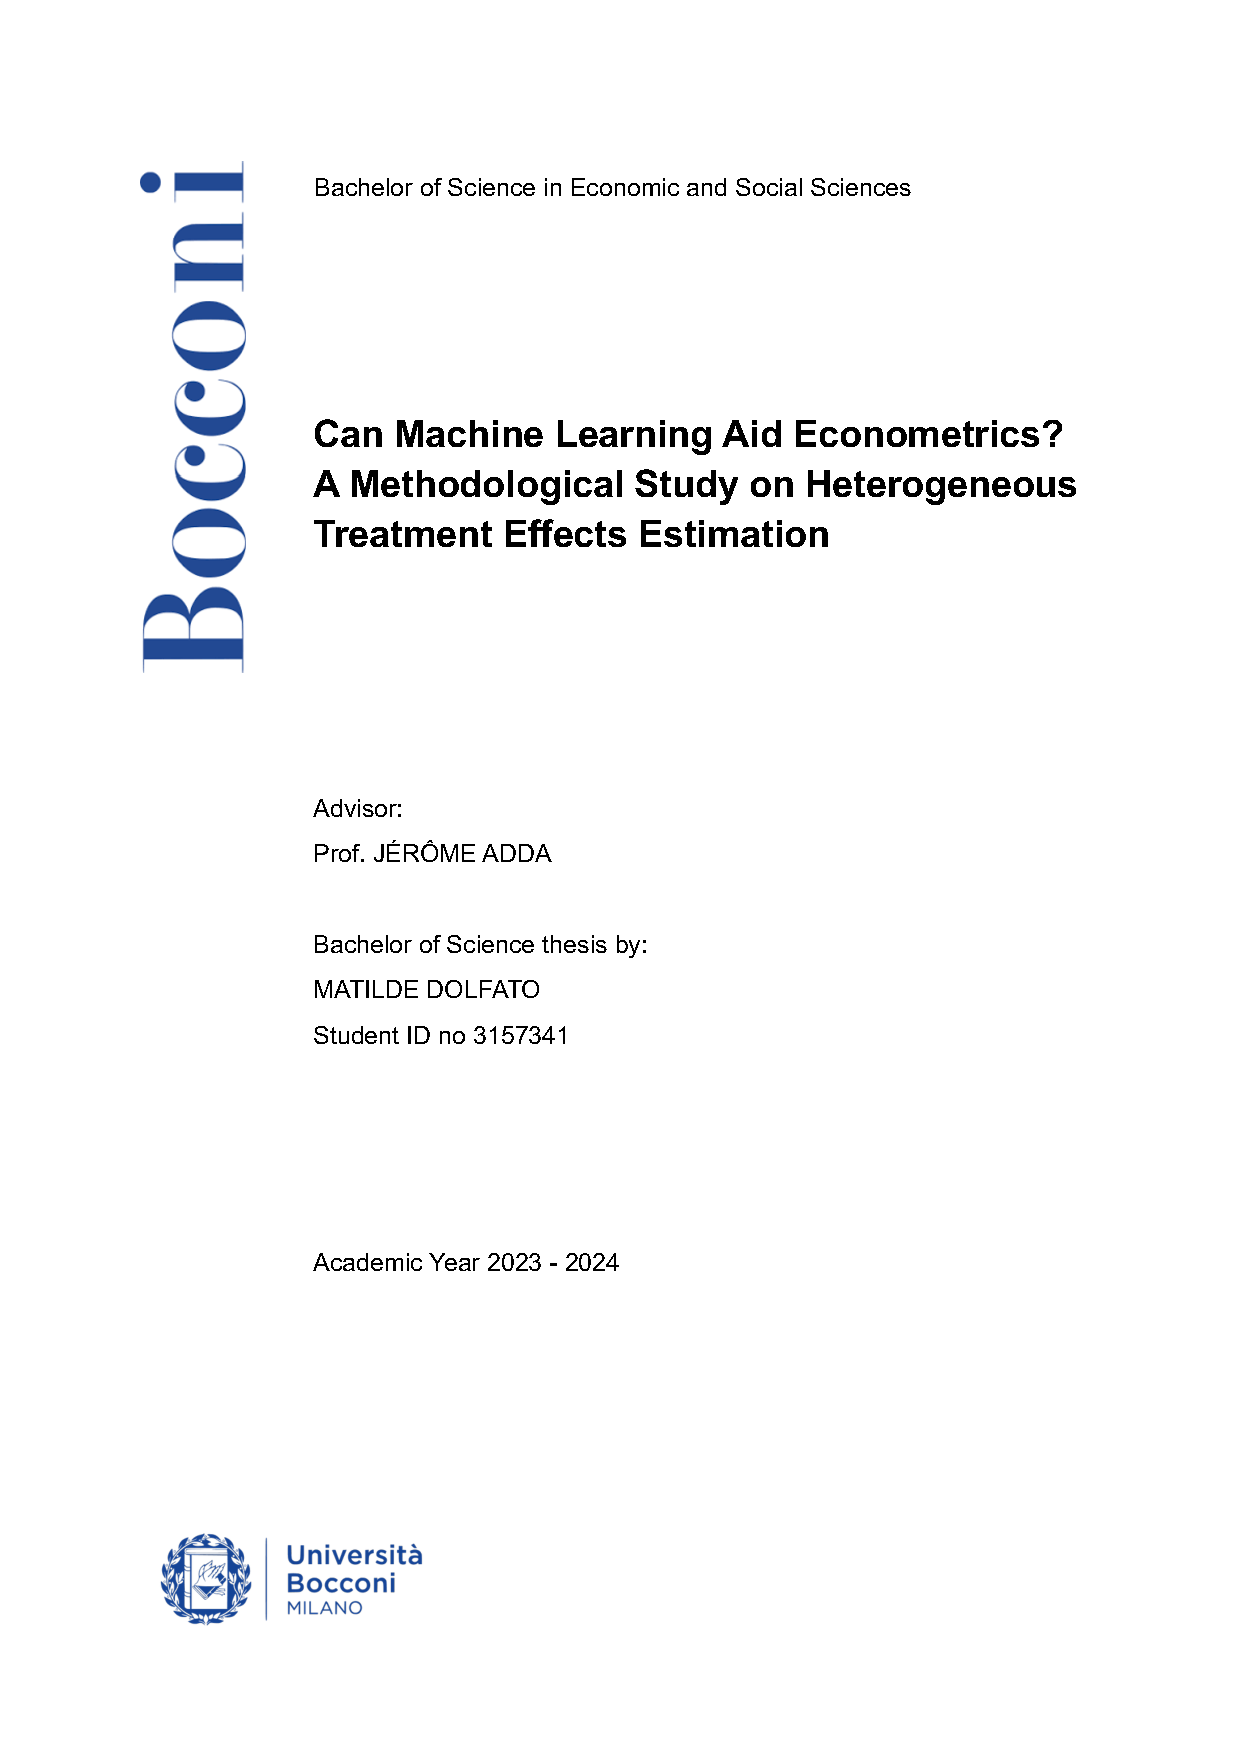
\includepdf[pages=-]{frontespizio_matildedol.pdf}

\sloppy

%% title page (sbagliata)
%\include{titlepage}

%% empty pages
\pagenumbering{roman}
%\renewcommand{\thepage}{\Roman{page}}
\setcounter{page}{1}
\newpage
\thispagestyle{empty}
\mbox{}
\newpage
\thispagestyle{empty}
\mbox{}

% %% abstract + blank page
% \clearpage
% \thispagestyle{empty}
% \thispagestyle{plain}
\begin{center}
\large{\textbf{Abstract}}
\end{center}

The study of policy effects is core in empirical economic research. The effect of a policy is likely to vary across different units of a population. Recently, many approaches to estimate heterogeneous treatment effects have been proposed in econometrics, also touching upon the machine learning field. This has triggered the emergence of causal machine learning, and empirical economists have diverging opinion on whether it should be used. The main contribution of this study is to provide an exhaustive methodological review on the estimation of heterogeneous causal effects. Moreover, it investigates the impact of causal machine learning on econometrics, attempting to answer the question of whether and how it can be beneficial. It is found that the main methods to estimate heterogeneous effects are: including interactions in a linear regression; the marginal treatment effect estimator; matching on propensity scores; local regressions with differencing; double machine learning; and causal forests.  
Moreover, I argue that machine learning can be beneficial to econometrics, especially as it flexibly models data and can be adapted to accurately estimate causal effects, and therefore it should be integrated in this discipline. 
% \clearpage
% \thispagestyle{empty}
% \mbox{}

%% acknowlegments 
\clearpage
\thispagestyle{empty}



\textit{A special thank to professor Jérôme Adda, who inspired me everyday in class, and taught me something that is found in this thesis, and goes way beyond it. 
}
\\

\textit{I thank professor David Rossell, who first sparked in me the curiosity for machine learning and helped crafting the idea for this thesis, and Lorenzo M, who gave me precious suggestions on these matters and much more. }

\textit{I am also deeply grateful to professors Massimo Marinacci, Maristella Botticini and Chiara Fumagalli: I am honoured to say that you gave me some advice I will always keep with me. }\\

\textit{A heartfelt thank to my friends Lucrezia, Bianca, Ilaria, Lorenzo G, Francesco S, Francesco D, Luigi, Federico, Gabriele N, Alessandro, Zoe, Michelle and Gabriele P. You made these three years better than I could have ever imagined. Thank you for keeping me going every time I don't see how or don't know where to go; I found in you another home.}

\textit{
Thank you also to my best friends Chiara, Roberta, Celeste and Anna, who will always remain such, no matter where life brings us.}

\textit{My last thanks to Elisa and Paola, without whom I sincerely think I would be completely lost. You are my role models and I feel incredibly grateful to have you by my side and be by yours for all the life to come.}\\


\textit{This thesis is dedicated to my parents Giovanna and Fabio, the best team I know. You give me an incredible strength to navigate life, while reminding me not to take it too seriously.}




%% blank page
\clearpage
\thispagestyle{empty}
\mbox{}

%% TOC
\clearpage
\thispagestyle{plain}
\tableofcontents

%% blank page
\clearpage
\thispagestyle{empty}
\mbox{}

%% begin text
\clearpage
\pagenumbering{arabic}
\setcounter{page}{1}
\begin{doublespacing}
\chapter*{Introduction}
\addcontentsline{toc}{chapter}{Introduction}
\markboth{INTRODUCTION}{}

The study of policy effects is core in empirical economic research. A major part of this discipline is concerned with investigating how a certain policy, called treatment, affects a population (of individuals, firms, countries, etc.), by measuring the causal relationship between such treatment and a certain variable of interest. The econometric literature provides a wide range of methods to estimate the treatment effect on a population on average (some collections are \citealp{angrist2009mostly}; \citealp{imbensrubin2015}; \citealp{hernanrobins2023}). The effect of a policy, however, is likely to vary across different units of a population, probably at the individual level. This variation is due to individuals differing in many characteristics, that determine how they react to a policy, and that they may self-select into treatment. Estimating the \textit{heterogeneous} effects of the policy, at least for some subgroups of the population, is crucial for social policy. In fact, if policymakers have information on which subgroups benefit the most from a treatment, they can choose more effectively to which part of the population and to which extent the treatment should be applied, allocating resources more efficiently (\citealp{heckman2005structural}; \citealp{xie2012estimating}; \citealp{zhouxie2020heterogeneous}). 

The econometric literature on heterogeneous causal effects estimation, however, has not a long history, and methods to perform this task have been proposed only quite recently. This may be due to the inferior availability of data and precise individual-level information that there was in the last century, compared to today (\citealp{wagerathey2018}). 
In fact, the pioneer of these methods is \citet{imbensangrist1994}'s Local Average Treatment Effect (LATE) estimator. It is an Instrumental Variables (IV)-based method, which estimates the policy effect only for a subgroup of the population, those who comply with a change in the instrument.
The Nobel Prize in Economic Sciences \footnote{More specifically, the ``Sveriges Riskbank Prize in Economic Sciences in Memory of Alfred Nobel''.} to G. Imbens and J. Angrist in 2021 (together with D. Card) particularly honours this significant breakthrough in econometrics (\citealp{lechner2023}).
Indeed, the LATE estimator paved the way for the development of other methods to estimate heterogeneous treatment effects, and since then novel advanced approaches have been proposed. Among these, there are both structural models developing on the IV approach (e.g. \citealp{heckman2005structural}), and others using trending statistical techniques like non-parametric methods (e.g. \citealp{nie2021quasi}; \citealp{xie2012estimating}). 

These advancements in econometrics have also touched upon the computer science and machine learning fields. Machine learning is a subfield of artificial intelligence, that develops algorithms to be applied to data, mainly for tasks of prediction and classification. These disciplines have come to the forefront in the last decades, bringing profound technological improvements, also tied to the access to larger datasets and greater computational capabilities of recent times.  Indeed, economists have been using methods that typically belong to machine learning for economic research. Most recently, they are also adapting them to the specific case of causal inference, developing the new area of research of \textit{causal} machine learning (\citealp{athey2019}; \citealp{efron2020prediction}; \cite{articleml}; \citealp{lechner2023}).\footnote{Throughout this thesis, I use ``causal machine learning'' and ``machine learning for causal inference'' or ``for empirical economic research'' as synonyms.} In fact, the estimation of heterogeneous causal effects appears to be one of the most suitable econometric tasks for the application of causal machine learning tools (\citealp{curthetal}; \citealp{videoimbangr}). 


%THE FIELDS ARE DISTINGUISHED BUT THE ALGORITHMS ARE SIMILAR AND SHARE THE SAME ROOT, as pittura classica 400centesca e il puntinismo impressionista che usano gli stessi colori in modi diversi :D 

However, the use of causal machine learning is not embraced by all empirical economists. Some of them strongly support it for the prediction accuracy and computational capacity of machine learning algorithms, while others are more cautious and skeptical about its suitability for economic studies. 

For instance, in an interview by I. Andrews in May 2022, the Nobel Laureates that contributed so much to the advancement in econometric methodology themselves, G. Imbens and J. Angrist, expose sharply diverging opinions on the impact of machine learning on economics (\citealp{videoimbangr}). Another example are J. Heckman and R. Pinto, who in a paper comparing some methods from econometrics and computer science, conclude that ``\textit{Economics has a rich body of theory and tools to address policy problems. Applied economists today would do well to use the impressive body of tools embodied in modern structural econometrics}'' (\citealp{heckmanpinto2022}). S. Athey and G. Imbens, on the other hand, present an overview of machine learning methods relevant to economics, and state that the list of tools they discuss ``\textit{should be part of the empirical economist’s toolkit and should be covered in the core econometrics graduate courses}'' (\citealp{atheyimbens2019}).

As it is evident, a vivid debate is currently underway among the economic academia, and although it is not possible to go back in time and completely deny the use of machine learning, the way in which it can affect empirical economic research is still an open question. \\

In light of this scenario, the aim of this study is to clarify the recently developed array of methods available to economists for estimating heterogeneous causal effects, combining econometrics and machine learning. 
Furthermore, this thesis seeks to understand what are the roots of the two opposing views on the use of causal machine learning. By doing so, it intends to contribute to answering the question of whether and how machine learning can actually benefit empirical economic research, especially in the case of heterogeneous treatment effects estimation.

Among similar methodological surveys there are, for the econometric part, \citet{xie2012estimating} and \citet{zhouxie2020heterogeneous}, and for the machine learning side, \citet{gongetal}; \citet{Knaus_2020} and part of \cite{athey2019}. Moreover, there are works comparing the two approaches, like \citet{dorie2019automated} and \citet{heckmanpinto2022}, but concerning the estimation of the average treatment effect and considering rather specific algorithms. Hence, the main contribution of this study is to combine the two fields and provide an exhaustive overview of all the fundamental methods economists have to estimate heterogeneous causal effects, and also to assess whether the machine learning ones can be advantageous for this task. \\

The rest of this thesis is organized as follows. First, the next section explains some basic concepts and algorithms to ease the understanding of the following technical analysis and discussion. Chapter \ref{chap1} concerns the methodology review and explains each method in detail. Chapter \ref{chap2} investigates how causal machine learning methods relate to econometric ones and what are their potential gains, and looks at some empirical evidence from the literature to assess how they perform for heterogeneous effects estimation.



\section*{Preliminary Concepts} \label{prelconc}
\addcontentsline{toc}{section}{Preliminary Concepts}

The general setting considered throughout this thesis is that of an observational study on a sample of $n$ individuals, each one denoted by $i$. Some of these are exposed to a treatment $D$, distinguishing the ``treatment'' group ($D=1$) and the ``control'' group with ($D=0$), to which no treatment (or in a more general setting, for other values of $D$, a different one) is applied. We study the effect of the treatment on an outcome variable of interest $Y$ given a set of $J$ individual characteristics $X$. We further denote $Y_1$ the potential outcome for the treated individuals ($D=1$), and $Y_0$ the potential outcome for control individuals ($D=0$). We indicate in lowercase the realizations of a variable, and with a hat the estimates. For instance, $y$ is a realization of $Y$, and $\hat{y}$ is an estimate. 

In general, treatment effects are estimated as the difference in outcomes between treated and non treated units, after controlling for the characteristics $X$ to ensure comparability between the groups (\citealp{imbenswooldr2008}). \\

Furthermore, some approaches to studying policy effects assume that the treatment is exogenous. The exogeneity (or ignorability) assumption states that the treatment is independent of potential outcomes given $X$, i.e.
\begin{equation}
    (Y_1, Y_0) \independent D | X \,\, \footnote{I refer to the notation used by \citet{xie2012estimating}.}
    \label{eq:exog}
\end{equation}    

Violations of this assumption are given, for instance, by individuals self-selecting into the treatment, that is one of the source of heterogeneity in policy effects, besides individuals reacting differently to the treatment (\citealp{zhouxie2020heterogeneous}). 

\paragraph{\scshape Propensity Scores} \label{ps}Many methods to estimate heterogeneous treatment effects (HTE henceforth) presented in this study are based on propensity scores.
Let us define propensity scores as the probability of an individual in the sample of receiving the treatment, given their characteristics $X$, i.e. 
\begin{equation}
    P(X) \equiv Pr(D=1|X) \,\, \footnote{I refer to the definition used by \citet{xie2012estimating}, even though this definition of propensity scores is generally used and accepted.}
\end{equation}

\citet{rosenbaum1983central} crucially found that under exogeneity, it is sufficient to condition on propensity scores $P(X)$ to estimate HTE. So, the assumption in equation \ref{eq:exog} becomes 
\begin{equation}
    (Y_1, Y_0) \independent D | P(X)
\end{equation}

In fact, propensity scores allow to summarize the relevant information in the possibly high-dimensional covariates $X$ ($n \times J$) in a lower dimensional variable $P(X)$ ($n \times 1$), to more easily balance covariates and ensure comparability of the units between the treatment and control group. 

\refstepcounter{intropara}\label{kernel}
\paragraph{\scshape Kernel Regression} 
The kernel regression is a specific type of local regressions. Local regressions are, in general, non-parametric statistical methods that estimate the outcome $Y$ \textit{locally}, allowing for a non-linear relationship between the covariates and the outcome. The idea is to estimate the outcome $y_i$ as a weighted average of the outcomes of the observations ``close'' to $i$, meaning with values of $X$ in a neighbourhood of $x_i$.\footnote{For simplicity, assume that here $X$ contains only one variable.} The kernel regression uses a specific weighting function, the kernel, in this algorithm. 

More specifically, following the lines of \citet{Ullah2016}, say we want to estimate the function $\mu(X)$, where
\begin{equation}
Y = \mu(X) + U
\end{equation}
with $U$ being the random error component. We do so by modelling $\mu(x)$ locally at a given $x$, applying a linear regression to the data \textit{close} to $x$. This means that we consider the linear regression
\begin{equation}
y_i = \alpha (x) - (x_i - x)\beta(x) + u_i
\end{equation}
for each $x_i$ with $i=1,...,n$ to determine the local regression function $\alpha(x)$ for $Y=y$ at $X=x$. The local linear regression method leads to the minimization problem 
\begin{equation}
    \text{min} \sum_{i=1}^{n}{(y_i - \alpha (x) - (x_i - x)\beta(x))^2 \,\, K\left(\frac{x - x_i}{h}\right) }
\end{equation}
where $K(\cdot)$ is the kernel weighting function. It is a decreasing function of the distances of $x_i$ from the point $x$, with $h$ being the bandwidth that determines the amount of local information used to determine the estimated outcome $y$. By solving the minimization problem, we obtain the estimated regression function for $Y$ at $X=x$, 
\begin{equation}
    \hat{\mu}(x) = \hat{\alpha}(x)
\end{equation}
and $\hat{\beta}(x)$ is the local slope. Iterating this process for each $x$ in $X$ we estimate a smoothed curve of the outcomes $Y$.

\paragraph{\scshape Regularization, Over Fitting and Cross-Validation} \label{regofcv}

In general, machine learning algorithms intrinsically perform \textit{regularization}. Regularization is the automatic selection of relevant covariates performed by statistical methods, reducing errors caused by \textit{over fitting}. Over fitting, on the other hand, occurs when a model fits the data too closely, hence it is unable to make accurate out-of-sample predictions and leaves little to the interpretation of causal relationships. Selecting covariates implicates reducing the variance of the estimates and also the risk of over fitting, but possibly biasing the results (as some information is ``missing''). Hence, this creates a tradeoff between bias (regularization) and variance (over fitting), which are in general inherently balanced by machine learning algorithms. 
The next two paragraphs provide technical examples of how this mechanism works. 

Furthermore, \textit{cross-validation} is a technique used in machine learning to evaluate the performance of a model and provide for over fitting. In brief, it consists in dividing the sample in multiple subsamples, or folds, and using some of them to train the model, and the rest of them (generally, only one) to test it. This procedure is repeated many times, each time with a different test set (\citealp{Refaeilzadeh2009}). 


\paragraph{\scshape LASSO Regression}\label{lasso}
The Least Absolute Shrinkage and Selection Operator (LASSO) regression (\citealp{tibshirani1996regression}) is a regularization technique typically used in machine learning. It adds a penalization term to the residual sum of squares of the regression, to inherently select the variables.

More specifically, to visualize how it works we look at the logit version of the LASSO, as presented by \citet{goller2020does} for propensity scores estimation (see Method \ref{match}). 

Consider the minimization function 
\begin{equation}
    \underset{\beta}{\text{min}} \,\, \Biggl\{ \sum_{i=1}^{n} \bigl[ -d_i x_i \ + \log (1 + \exp (x_i \tau)) \bigr] + \lambda \sum_{j=1}^{J} |\tau_j| \Biggr\} 
\end{equation}
where $d$ is an observation of the treatment variable $D$, and $\tau$ is the coefficient measuring the relationship between the covariates $X$ and the treatment. The first summation term corresponds to the residual sum of squares, while the second one is the penalization term, controlled by $\lambda$. This corresponds to the bias that will result in the estimates. By adding this term, the absolute value of the coefficients $\tau_j$ is shrank towards 0, reducing their importance or altogether eliminating them from the model, resulting in an automatic model selection.

Indeed, as $\lambda$ increases, the penalization term will be higher and the regularization will be more stringent. Hence, the estimates will have a lower variance and a larger bias. So, the value of $\lambda$ controls the tradeoff between variance and bias, and its choice is crucial. The optimal choice of the $\lambda$ is based on data, generally with a cross-validation technique. 




\paragraph{\scshape Random Forests}\label{rf}
Random forests (\citealp{breiman2001random}) are a machine learning non-parametric and non-linear estimation technique. They are constructed on
regression trees (\citealp{breiman2017classification}), which are a specific version of decision trees where the variable to be predicted is numerical. Decision trees, in general, are a common machine learning algorithm that recursively splits the covariate space into intervals, while minimising the error in the prediction of the outcome variable. The final structure is a rotated tree, where the initial trunk contains all the data, and each branch corresponds to a split of the observations defined by a certain threshold or value (for categorical variables) of one or more covariates. At the end of the splitting procedure, in the final nodes (leaves), the predictions are given as the average of the outcomes of all the observations included in that leaf.\footnote{In simple words, an example of two branches with $X$ being age and gender is: \textit{for male individuals (branch 1), if they are older than 25 (branch 1.1), we predict $\hat{y_1}$; if they are younger than 25, $\hat{y_2}$ (branch 1.2); for female individuals (branch 2), if they are older than 40 (branch 2.1), we predict $\hat{y_3}$; if they are younger than 40, $\hat{y_4}$ (branch 2.2)}.}  


A random forest is an ensemble of regression trees, meaning that it combines the output of multiple trees, built on different random subsets of the covariate space. In fact, the final model is obtained through an average of the many trees, to increase the accuracy of the prediction.\footnote{Notice that the accuracy of a prediction is defined as the combination of (the opposite of) both its bias and its variance (\citealp{walther2005concepts}). This concept is crucial and should be kept in mind for the subsequent discussions in this study.}

In random forests, the balance between bias and variance is controlled by the deep to which each tree is developed - in other words, by the number of observations in the final nodes used for each prediction. A higher number of observations in the leaves determines a lower variance and a higher bias of the prediction. In fact, it indicates that less splits have been made, and thus that intuitively the prediction is more ``coarse''. This mechanism, together with averaging between many trees to obtain the final forest, entails the automatic selection of the variables and controls over fitting (\citealp{athey2019}; \citealp{goller2020does}). 


\chapter{Estimating Heterogeneous Treatment Effects} 
\chaptermark{ESTIMATING HET. TREATMENT EFFECTS}
\label{chap1}{}

This chapter pursues the first aim of this study, that of providing a survey of the main methods used by economists to estimate heterogeneous causal effects, combining classic econometrics and newly proposed causal machine learning methods. Before delving into the technical review in Section \ref{meth}, Section \ref{over} provides an overall idea of the methodological scenario. 


\section{An Overview} \label{over}

There is a diverse group of methods to estimate heterogeneous causal effects, that differ substantially from one another yet share some basic features and are related to each other.\\

First, there are regression-based methods (\ref{interact}, \ref{mte}, \ref{locreg}), which either assume to include all the relevant individual characteristics (under the exogeneity assumption) or consider unobservables that could in part drive the heterogeneity, using an IV approach. This is the case of the marginal treatment effect (MTE) estimator by \citet{heckman2005structural}, which is based on a specific structural model. 
Alternatively, the idea behind regression-based methods is that we need to allow for non-linearities in the relationship between the response variable and the treatment, to obtain heterogeneous causal effects. Some econometric ways to do so are including interactions in a linear regression (for instance, discussed by \citealp{zhouxie2020heterogeneous}) and the commonly used non-parametric local regressions (\citealp{ferwerda2015krls}; \citealp{hastie2009elements}; \citealp{huber2023causal}; \citealp{imbenswooldr2008}; \citealp{shim2009kernel}).

Then, other methods consider matching the units between the treatment and control groups based on similar characteristics $X$ (\ref{match}), to ensure the comparability between the units and estimate treatment effects based on this comparison (e.g. \citealp{abadieimbens2016}; \citealp{xie2012estimating}). 

In addition to this, some of these methods use propensity scores, as proposed by \citet{xie2012estimating} (\ref{match}, \ref{locreg}). Propensity scores replace the covariates $X$ as balancing measure (for instance, in a regression), because they summarize the relevant information of the individuals in a lower-dimensional parameter easier to use, as explained in the \customref{ps}{related paragraph} above.
 

Finally, there are two main uses of machine learning for HTE estimation. First, \citet{cannas2019comparison}; \citet{goller2020does}; \citet{lee2010improving} and \citet{mccaffrey2004propensity}, among others, propose to use algorithms from machine learning to perform the first-stage estimation of propensity scores, thus as an auxiliary, possibly complementary tool to econometric methods (like Methods \ref{match} and \ref{locreg}). Secondly, economists have been using off-the-shelf causal machine learning algorithms (Methods \ref{dml}, \ref{cf}), that entirely substitute traditional ones (some examples are \citealp{atheyimbens2015}; \citealp{atheyimbens2016}; \citealp{wagerathey2018}; \citealp{atheytibishirani}; \citealp{chernozhukov2018double}; \citealp{rulensem}).
Among others, \citet{athey2019}, \citet{huber2023causal} and \citet{lechner2023} discuss the use of these methods for HTE estimation.  

\section{The Methods} \label{meth}

In brief, the methods to estimate HTE presented in this study are: a linear regression with interaction terms; the MTE estimator by \citet{heckman2005structural}; a matching algorithm that then smooths the estimated effects; a local regression applied to the treatment and control group, with differencing; the double machine learning algorithm by \citet{chernozhukov2018double}; and the causal forests algorithm by \citet{wagerathey2018}. 

Also some insights on how each method relates to the others and when it is most suitable are given. 

\subsection{Including Interactions in a Linear Regression} \label{interact}
The most simple way of estimating HTE is to include interactions terms between the treatment and the covariates in a basic linear regression. Indeed, if we linearly regress $Y$ on the treatment $D$ and the individual characteristics $X$, the coefficient of the treatment variable will give us an estimate of the average treatment effect (ATE), as it is equal to $ \hat{Y_1} - \hat{Y_0}$. 
We shall include in the regression an interaction term $X_j \cdot D$, with $j \in [0, ..., J]$, where $X_j$ is a categorical variable or a discretized one with $K$ groups or intervals, across which the treatment effect is expected to vary. The resulting regression is

\[
Y = \alpha + \beta X + \delta{_0} D + \delta{_j} X_j D + \epsilon
\]

Estimating it will give us an estimate of the treatment effect for each category in $X_j$. The k-th  estimate of the HTE will be equal to $\delta{_0} + \delta{_{j,k}} $, with $k = 1,..., K$. \\

The main drawback of this method is that it assumes linearity in the relationship between the outcome $Y$ and the treatment and covariates, which could bias the results (\citealp{zhouxie2020heterogeneous}). Moreover, it requires to know a priori which is the individual characteristic responsible for the heterogeneity, and this needs to be categorical or to be discretized. So, the method is a good solution for small and simple datasets, providing very clear results, but it is not suitable for more complex studies. 


\subsection{Marginal Treatment Effect Estimator} \label{mte}
The marginal treatment effect (MTE) estimator proposed by \citet{heckman2005structural} is a novel and advanced version among the IV approaches, implementing a \textit{local} IV. It generalizes the ATE and LATE estimators, as they can be obtained as a weighted average of the MTE.
The model on which the MTE is based combines treatment effect literature with structural estimation. Indeed, it allows for the selection into treatment to be determined by a decision rule (structural part), and this choice, as well as potential outcomes, can be influenced also by unobservables, relaxing the exogeneity assumption.
Here, the MTE method is explained on the lines of \citet{carneiro2011estimating}. \\

First, consider the regression

\begin{equation}
    Y = \alpha + \delta D + \varepsilon
\end{equation}

where $\delta$ is the effect of the treatment on the outcome. Define potential outcomes as
\begin{equation}
\begin{split}
    Y_1 = \mu_1(X) + U_1,\\
    Y_0 = \mu_0(X) + U_0
\end{split}
\end{equation}
where $U_1$, $U_0$ are the unobservable components influencing potential outcomes and $Y_1 - Y_0 = \delta$. Furthermore, consider the latent variable choice model 
\begin{equation}
    I_D = \mu_D(Z) - V
\end{equation}
and the decision rule 
\begin{equation}
    D = 1 \,\, \text{if}\,\, I_D \ge 0; \,\,\,\, D=0 \,\,\text{ otherwise}
\end{equation}

Notice that the unobservable component in the choice model $V$ collects unobserved effects that make the individual \textit{less} inclined to be treated, and define
\begin{equation}
    U_D \equiv F_V(V)
\end{equation}
where $F_V$ is a strictly increasing function.
Then the propensity scores $P(Z)$ are estimated with the instrument $Z$, getting
\begin{equation}
    P(z) \equiv Pr(D=1 | Z = z) = F_V(\mu_D(z))
\end{equation}
Finally, the MTE, defined as 

\begin{equation}
    \text{MTE} (x, u_D) \equiv E(\delta | X = x, U_D = u_D)
\end{equation}

can be estimated as a function of propensity scores and the unobservables. Indeed, we consider the case in which the propensity score equals the value of the unobservable component, $p = u_D$, i.e. when the individual is indifferent between being treated or not. So, we are able to estimate the MTE for the indifferent individuals at different values of the propensity score, as
\begin{equation}
   \text{MTE} (x, p) = \frac{\partial E(Y|X = x,P(Z) = p)}{\partial p} 
\end{equation}
for $P(Z) = p$ and $X=x$. Indeed, $P(Z)$ is referred to as a local IV. The group of individuals who are indifferent between being treated or not, for which we estimate the MTE at different values of the propensity score, are the relevant ones policy-wise, because they are the ones who, at the margin, would change their mind if treated, and let us estimate the optimal extent to which the policy should be applied. \\

Compared to the others, this method is a more structural approach and it relaxes the exogeneity assumption, which most likely does not hold in reality. This allows for a greater economic interpretability of the results and to apply the method to more datasets and studies. Alongside this, \citet{zhou2016propensity} discuss in detail the differences between the following propensity scores-based methods (\ref{match} and \ref{locreg}) and the MTE, also finding that the former two are valid even under some violations of exogeneity, partly decreasing the distance between the applicability of the two approaches.

\subsection{Matching on Propensity Scores} \label{match}

Matching is a non-parametric statistical technique that directly compares (groups of) units to estimate heterogeneous treatment effects as the difference in their outcomes, for each match. \citet{xie2012estimating} propose to use propensity scores to match the units and then smooth the resulting estimates of the treatment effects. 

An intuitive idea of the rationale behind this method is provided by \citet{d1998propensity}. Individuals in the two groups with equal propensity scores have equal probability of being treated or not, as if they were randomized into either of the two groups. Randomized experiments, in fact, entail to randomly assign units to the treatment and control group, ensuring that on average there are no systematic differences between them. Thus, matching units on their propensity scores allows to directly compare the outcomes of each match of treated and non treated individuals and estimate the treatment effect.  

The algorithm works as follows. First, it requires to estimate $P(X)$ and to match treated and non-treated units with the 1:1 matching framework.\footnote{See \citet{xie2012estimating} for more detail on the many matching types and algorithms that can be used.} Then, it computes estimates of the HTE as the difference in the outcomes of each pair of units, $\Delta y = y_1 - y_0$, getting individual-level information on the treatment effect. Finally, we fit a local regression of $\Delta y$ on $\hat{P(X)}$, to obtain a smoothed curve of the treatment effect heterogeneity. 

The first-step estimation of propensity scores can be performed with many algorithms. A traditional approach is to use a logistic regression, as in \citet{xie2012estimating}. Alternatively, more advanced algorithms like a \customref{lasso}{LASSO regression} or \customref{rf}{random forests} can be used, as in \citet{goller2020does} and \citet{Knaus_2020}. The implications of the choice of the algorithm to predict propensity scores are discussed in the next chapter, in Section \ref{disc}. 




\subsection{Local Regression with Differencing} \label{locreg} 
Another option economists have is to use local non-parametric regressions on propensity scores, as presented by \citet{xie2012estimating} as ``\textit{Smoothing - Differencing method}''. The fundamental concept behind this method is to use a local regression to allow for a non-linear relationship between the covariates and the response variable, as explained in the paragraph on the \customref{kernel}{kernel regression}. 

In fact, the first step consists in estimating $P(X)$, with the algorithms discussed for Method \ref{match}. Then, we fit two local regressions of the outcome $Y$ on $\hat{P(X)}$ for the treatment and control groups separately, getting two smoothed curves of the fitted values. Finally, we take the difference between the two regression lines over the common support of $\hat{P(X)}$, to get the estimates of HTE for each value of the propensity score. \\

This approach can be considered as an extension of the interactions Method \ref{interact}. Indeed, including interactions in a linear regression is a way of allowing for a piece-wise linear relationship between $D$ and $Y$, where the slope (the estimated coefficient) can change at different values of $X_j$ (the variable giving the heterogeneity). Local regressions extend this idea in a non-parametric form, allowing for a non-linear relationship over the whole range of $X$, so they relax further the functional assumptions on the relationship between $Y$ and $D$. A further development of this approach are machine learning algorithms that are based on interactions, like causal forests by \citet{wagerathey2018} that are presented below (Method \ref{cf}).


\subsection{Double Machine Learning} \label{dml}

The first off-the-shelf causal machine learning method is double machine learning (DML), first proposed by \citet{chernozhukov2018double}.

The concept at the heart of this method is not far from the idea explained at the end of Section \ref{match}, i.e. combining machine learning and econometric methods, using the former to estimate nuisance parameters.\footnote{Nuisance parameters are a subset of the parameters of a model (here, propensity scores and potential outcomes) that are needed for the model specification, but only in order to estimate other parameters, the ones which we are interested to inference (here, the treatment effects).} However, these estimates may be biased, as explained in the paragraph on \customref{regofcv}{regularization} and further discussed below (Section \ref{disc}). Indeed, DML is a more complete algorithm that uses a \textit{doubly robust} approach and an orthogonal estimator of treatment effects to provide unbiased treatment effect estimates. Doubly robust methods (see for reference \citealp{huber2023causal}; \citealp{kennedy2023}) propose estimators that are a function of both propensity scores and potential outcomes, thus requiring that either one of the two models is correctly specified, being more robust to model mis-specification (and biased estimates) than previously discussed methods. 


Technically, the DML method consists in a two-step estimation of treatment effects. First, we estimate the (potentially) high-dimensional propensity scores and potential outcomes using algorithms from machine learning (again, like a \customref{lasso}{LASSO regression} or \customref{rf}{random forests}). Then, we plug the residuals from these estimations in a residual-on-residual regression, obtaining a score function that is Neyman orthogonal, thus it is not sensitive to the possible biases in the nuisance parameters estimates. Lastly, it uses cross-validation techniques to correct for over fitting. 

Finally, for what regards the second-stage model to estimate the treatment effect, the DML approach has been analyzed in multiple papers in the literature. The original paper \citet{chernozhukov2018double} considers the case of estimating the ATE or a low dimensional LATE. Instead, in the specific case of HTE estimation, the online article \citet{towardsds} proposes to use an interaction model in the second step to allow for non-linear relationships, so it would be an evolution of Method \ref{interact}. \citet{huber2023causal} suggests to regress the score function defining the ATE on $X$ or on a subset of it to get an estimate for HTE.
\citet{nie2021quasi} considers the case in which the function identifying treatment effects can be modeled through a kernel regression, and thus augment Method \ref{locreg} above. 
Lastly, \citet{wagerathey2018} models treatment effects with a causal forest, which we present in the next section.

\subsection{Causal Forests} \label{cf}
Another causal machine learning method to estimate heterogeneous treatment effects are causal forests, proposed by \citet{wagerathey2018}. Causal forests are an adaptation of the common machine learning algorithm of \customref{rf}{random forests} to causal inference. In causal forests, briefly, the ``leaves'' of each tree give the estimates of causal effects rather than estimates of the outcome $Y$. The splitting algorithm, in fact, maximizes the heterogeneity in the treatment effect, instead of minimizing the prediction error as in random forests. Thus, the estimated treatment effect varies across different values of the covariates in $X$. Moreover, the algorithm is ``honest'', in the sense that for each \textit{causal} tree, the sample used for prediction is different from the samples used to build the trees and split the covariate space. \\

Indeed, causal forests can be seen as a machine learning version of allowing for non-linearities in the relationship between $X$ and $D$, and, in this view, a development of the interaction Method \ref{interact} and to some extent the local regression Method \ref{locreg}. As \citet{wagerathey2018} explains, in fact, this algorithm is close to kernels and matching in that they estimate the parameters as a weighted average of ``nearby'' observations, but they determine which observations receive more weight based on data, that is particularly important in complex and high-dimensional settings.  

\chapter{The Impact of Causal Machine Learning on Econometrics} \label{chap2}
\chaptermark{THE IMPACT OF CAUSAL MACHINE LEARNING}

Some of the methods presented come from the emerging area of causal machine learning. As suggested above, empirical economists have diverging opinions on its use, and what is the impact of (causal) machine learning on empirical economic research is still debated (\citealp{athey2019}; \citealp{bankarticle}; \citealp{dorie2019automated}; \citealp{heckmanpinto2022}; \citealp{videoimbangr}). 

This chapter aims at shedding light on whether and how machine learning methods can be used beneficially in empirical economic research. 

First, Section \ref{diff} presents how machine learning tools relate to econometric ones; then Section \ref{deb} dives into the potential gains and losses of machine learning for empirical economics, outlining the ongoing debate; lastly, Section \ref{disc} discusses in this regard the machine learning methods considered in the previous survey, using evidence from the empirical literature.


\section{Are They Even Different?} \label{diff}
%qui voglio dire che sono molto simili e quali differenze si possono pero individuare (high dim, preidction, interpretability) NON potential gains
S. Athey, while discussing the impact of machine learning on economics, questions if machine learning really needed a new name other than statistics (\citealp{athey2019}). 

In fact, the basic algorithms behind machine learning are not new to empirical economists, because they share the same root as statistical regression methods (\citealp{efron2020prediction}). Consequently, it is not always possible - nor necessary - to draw a line and classify each technique as either machine learning or econometric, as also arises from this study. For instance, the LASSO regression is widely recognized as a machine learning tool, but received some attention in the econometric literature before machine learning arrived in this field. Even more strikingly, the cross-validation technique is viewed as a fundamental part of machine learning algorithms, but has been historically used in economics, for example to determine the bandwith for a kernel regression (\citealp{athey2019}). \\

Having said that, there are some criteria on which machine learning methods can be distinguished from traditional econometric ones, and which justify the debate on their use.

First of all, methods from machine learning are tailored to handle very complex high-dimensional datasets, with a huge number of covariates and observations, compared to smaller datasets traditionally used in economic research (\citealp{bankarticle}; \citealp{efron2020prediction}).

Then, machine learning algorithms are focused on prediction, rather than on estimation (see \citealp{efron2020prediction} for a detailed explanation of prediction vs. estimation in general). This means that the concern of these methods is the goodness of fit of the model, and they aim at obtaining an accurate prediction of the outcomes (very high explanatory power). On the contrary, as causal relationships are the main interest of empirical economic research, classic econometric methods are focused on obtaining unbiased estimates of the causal effects between variables, at the cost of the goodness of fit of the model and of predictive accuracy of the outcomes (possibly low explanatory power). 
In fact, machine learning models generally include myriads of weak predictors, as opposed to econometric models that include only few strong explanatory variables.
Related to this, econometric models are based on statistical theory and the estimators they provide have asymptotic properties, meaning they are asymptotically normal and their results can be inferred to a whole population. This is crucial for economic causal inference, because for instance it allows to obtain confidence intervals and perform hypothesis testing. True values of real causal effects are generally not available, hence this property is particularly important to assess the quality of the estimation. Traditional (predictive) machine learning algorithms do not have such features, and therefore they are more suitable for simpler classification purposes, where a ground truth (the observed outcomes) is available (\citealp{athey2019}; \citealp{efron2020prediction}).

The last crucial point is that machine learning methods perform a data-based model selection, after a (large) set of covariates is provided by the researcher. This, intuitively, relates to the very high goodness of fit typical of these models. Also, this determines a tradeoff between over fitting and regularization, which machine learning algorithms intrinsically balance. Please refer to the paragraph on \customref{regofcv}{regularization and over fitting} for a more detailed explanation of this mechanism.
On the contrary, empirical economists generally specify only one model, then use all the data for the estimation, and inference the results based on statistical theory (\citealp{athey2019}). This is also related to the typically smaller size of datasets used with econometric methods, compared to machine learning ones.\\

Recently a new movement is emerging, combining machine learning algorithms with causal inference. The so-called causal machine learning is a new research area that is adapting machine learning tools to estimate causal effects (some leading examples are \citealp{atheyimbens2015}; \citealp{atheyimbens2016}; \citealp{atheytibishirani}; \citealp{rulensem}; \citealp{chernozhukov2018double}; \citealp{wagerathey2018}). In doing so, the objective is to harness the strengths of machine learning, while providing for some of the shortcomings these algorithms present when applied to economic research. For instance, \citet{wagerathey2018} adapt random forests providing causal forests with a tractable asymptotic theory and allowing statistical inference. In fact both causal forests and the DML method presented above belong to this movement (Methods \ref{cf} and \ref{dml}). Therefore, causal machine learning is likely to further narrow the distance between the econometric and machine learning traditions (\citealp{athey2019}; \citealp{lechner2023}).


\section{The Debate} \label{deb}

Based on the aspects that distinguish machine learning methods from econometric ones, some potential gains together with some limits of using machine learning in economic research arise; these outline the vivid debate going on among economists on this matter. \\

One of the arguments of economists that support the use of machine learning for empirical economic research is the data-driven model selection. In fact, it is more solid than classic procedures and it avoids economists' custom of checking alternative models ``behind the scenes'' (\citealp{athey2019}). Moreover, this property has many implications. 
It avoids imposing functional model assumptions, as the functional form is at least in part derived from the real distribution of data. Indeed, these algorithms flexibly model the (possibly complex) relationships between the variables. This also results in capturing non-linearities or other complex structures that could not be discovered in advance, and that traditional methods could fail to detect. This, for instance, is particularly relevant to detect heterogeneity in the policy effects (\citealp{bankarticle}; \citealp{mullainathanetal}).
In fact, S. Athey precisely maintains that regularization and automated model selection have several advantages on traditional methods and will likely become part of standard empirical practice in economics (\citealp{athey2019}).

On the other hand, economists who are reluctant about the use of machine learning bring the main, strong argument of interpretability. Being able to interpret the algorithm with which some predictions are obtained is crucial for economic research, that tackles questions on causal effects rather than prediction. Machine learning algorithms, however, are traditionally not interpretable, as the algorithm they use is not known in detail to the researcher and as they do not provide causal effects estimates. Moreover, the lack of a structural component in machine learning models impairs further interpretability of causal relationships (\citealp{heckmanpinto2022}; \citealp{videoimbangr}). 

However, causal machine learning algorithms overcome this hurdle, at least in part. This is because they are tailored to estimate causal effects and adapted to present asymptotic theory and perform causal inference, as explained at the end of the previous section. Therefore, they leverage the accuracy of the prediction and the flexibility typical of machine learning algorithms to produce accurate estimates of causal effects and aid econometrics in finding the correct functional form to achieve unbiasedness (\citealp{athey2019}). 

Finally, as explained above, machine learning algorithms are tailored to handle huge datasets, and especially for a number of covariates that is much larger than the number of observations. This feature could be void for economic studies, which are generally based on few covariates. For instance, in the specific example of estimating policy effects, getting effects estimates for very specific groups of the population identified by many characteristics could be useless and not actionable upon (\citealp{videoimbangr}). In fact, with simpler datasets classic econometric methods are sufficient, and machine learning ones do not appear to be useful (\citealp{bankarticle}). At the same time, nowadays there is an easier and easier access to datasets that are many orders of magnitude larger than before. Indeed, machine learning tools combined with newly available data sets could change economic research providing new questions, new
approaches, and more interdisciplinary works (\citealp{athey2019}). 
%metti che guido dice di usare ml quando c'è un botto di het

\section{Empirical Evidence} \label{disc} 
%qui voglio dire metodo per metodo i risultati, aggiungendo il discorso di var selection e che non serve interpretare in estimating PS, poi DML stessa cosa (anzi qui) e risultati, poi CF
The final question addressed now is how the specific methods considered in this study relate to the discussion on machine learning applied to economic research, and thus whether they improve heterogeneous causal effects estimation. \\

First of all, the machine learning methods considered overcome at least in part the non-interpretability argument discussed in Section \ref{diff}. Causal forests do so by presenting asymptotic properties. Also using machine learning for first-stage estimation of nuisance parameters, either with DML or as part of the matching or local regression methods, overcomes this limit. As explained by \citet{lechner2023} and \citet{lee2010improving}, in fact, in the first step we are not interested in the causal relationship between controls $X$ and the treatment or the outcome. 
In the second step, instead, we want to be able to understand the causal effect of the treatment on the outcome, and thus we implement traditional more interpretable econometric methods to estimate treatment effects.  \\

Furthermore, there is some empirical literature that compares machine learning algorithms to a logistic regression to estimate propensity scores. 

\citet{goller2020does} find that the LASSO regression performs particularly well compared to a logistic regression. Random forests, on the other hand, appear to lead to misleading results especially when the share of treated is low, possibly because the algorithm does not split deep enough to properly balance covariates.\footnote{With a small share of treated observations, splitting much the covariates space may easily lead to overfitting, as few (treated) observations would remain in each leaf.} Moreover, they conclude that since knowing a priori which of the many methods works best, implementing off-the-shelf causal machine learning algorithms like DML or causal forests could be more convenient. 
\citet{lee2010improving}, instead, find that ensemble methods, like random forests or an advanced version of regression trees, show the best performance in balancing covariates to then estimate effects, recommending them for propensity scores estimation. \citet{cannas2019comparison} provide similar results, preferring random forests to other machine learning algorithms and recommending them in place of logistic regressions to estimate propensity scores. 
Lastly, \citet{lee2010improving} find that the random forest algorithm performs better than others also for smaller datasets (with $n$ = 500). \\

Having said that, a matter to be addressed is the presence of a regularization bias in propensity scores estimates. Indeed, as explained in the paragraph on \customref{regofcv}{regularization and over fitting}, the inherent variable selection of machine learning algorithms enhances prediction accuracy, but possibly produces biased estimates. \citet{goller2020does} maintains that it is necessary to correct for this bias in propensity scores as it can translate to a higher bias in the treatment effect estimates. To this end, they implement a matching estimator with bias adjustment, but in the case of average treatment effect estimation. So, further work should be conducted to obtain HTE bias adjusted estimators, possibly on the lines of the matching or local regression algorithms (Methods \ref{match} and \ref{locreg}). 
At the same time, \citet{lee2010improving} consider that also econometric methods can lead to biased estimates if the modelling assumptions on which they are based are incorrect. Indeed, they compare a logistic regression without including interactions or non-linearities (powers of $X$) to many machine learning algorithms. They find that when the real data presents non-linearity, the logit model gives the highest bias;  also when there is linearity, its performance is comparable to that of some of the other methods. So, they implement the machine learning algorithms without correcting for the bias when estimating treatment effects. Thus, machine learning algorithms could possibly be implemented for first-stage estimation, jointly with the matching (\ref{match}) or local regression (\ref{locreg}) estimators for HTE, without the need of bias adjustment. \\

For what regards the DML and causal forests methods, there is not much empirical literature on comparisons to classic econometric approaches, especially for heterogeneous effects in economic studies. This may be because they are off-the-shelf causal machine learning algorithms substituting econometric ones, and also because they have been proposed very recently.

However, there are some papers that implement these algorithms for HTE estimation, with promising results. 

Two of the few examples for the DML algorithm are \citet{fuhr2024estimating} and \citealp{wangetal}. Both papers find that it gives more accurate results and that it fits non-linear relationships better than econometric methods. In the first paper, moreover, they state that structural analysis and assumptions are needed behind the application of this method, because it doesn't account for unobserved confoundness (as, for comparison, the MTE Method \ref{mte} does). 
Indeed, as discussed by \citet{lechner2023}, the upside of this algorithm is that it can be used as an helpful tool to human decision making, especially when combined with decision trees (or, equivalently, random forests), that clearly provide an idea of the criteria used by the machine learning algorithm, so that the human can understand it. 

Among the studies implementing causal forests, \citet{davisetal} find that causal forests identify treatment heterogeneity that other interaction approaches would have missed. \citet{bonanderetal} conclude that the method is suitable for estimating heterogeneity, but that one of its limits is that it performs poorly in low-dimensional datasets. 
Additionally, there are some papers in the medical literature comparing the performance of causal forests  to simple regressions. An example is \citet{elek2021regional}\footnote{It is a medical study, but given the limited number of covariates included (around 10) its results are relevant also for economic applications.}, that maintains that, compared to a full interaction linear regression model, the automatic selection of which variables give the heterogeneity performed by causal forests improves statistical power, and they are therefore preferred. \citet{venkatasubramaniam2023comparison}, instead, in a similar study conclude that causal forests should not be used alone, but always compared to classic regression methods, that in their evaluation performed better. \\

On the whole, it is found that the methods from the machine learning literature considered in this study allow for interpretability of the causal treatment effects, while harnessing the higher predictive accuracy of machine learning algorithms. Moreover, the empirical evidence shows that estimating nuisance parameters with machine learning gives more accurate results and better covariate balance, and both LASSO regression and random forests are preferred to a logistic regression for this task. Their performance, however, varies depending on the studies, and using off-the-shelf causal machine learning methods may be recommendable. These, in fact, appear to perform well for heterogeneous effects estimation, also detecting heterogeneity patterns that classic econometric methods miss. 

\subsection{Discussion}

From this study it arises that causal machine learning can bring fascinating improvements to empirical economic research. 
The main benefit it brings is the ability to model the data with highly flexible functional forms. This enables the researcher to discover hidden patterns of the relationships between variables, that are the basis of empirical economics questions. This is especially true for the investigation of heterogeneous causal effects, as the empirical results support. Furthermore, causal machine learning provides empirical economists with a solid model selection procedure based on data and very accurate estimations of causal effects. 

Alongside this, machine learning may also open new horizons for empirical economics, introducing new approaches and questions, possibly exploiting the abundance of very precise data available today.


It remains true that the methodological choice depends largely on the characteristics of the data and the study that is being conducted. Hence, the best choice is to integrate the two disciplines to leverage machine learning tools when they are most suitable, and use econometric ones when they are sufficient. Indeed, economic and statistical theory must remain the foundation of the model choice procedure. 

  
As a last consideration, it is evident that more work should be conducted in the direction of embodying machine learning in econometrics and empirical economics, as this integration presents some frictions. Nevertheless, even from the early steps taken so far, it is evident that causal machine learning can greatly contribute to econometrics, suggesting that this direction should be pursued further. 




\chapter*{Conclusions}
\addcontentsline{toc}{chapter}{Conclusions}
\markboth{}{}

Investigating heterogeneous policy effects is highly relevant for empirical economic research, and many methodological developments have been done in the last decades concerning this task (\citealp{zhouxie2020heterogeneous}). Not only, but heterogeneous effects estimation is also closely related to the recent advent of machine learning techniques in econometrics, which has triggered a vivid debate among experts on the use of \textit{causal} machine learning (\citealp{athey2019}; \citealp{videoimbangr}). 

In light of this, this study has first reviewed the main methods to estimate heterogeneous causal effects, combining the two disciplines, and then it has inquired whether and how causal machine learning can benefit empirical economic research. \\

In summary, the main methods economists have to estimate heterogeneous causal effects are: including interactions in a linear regression, mostly suitable for simple datasets; the marginal treatment effect estimator, a structural approach that allows for unobserved resistance to treatment (\citealp{heckman2005structural}); a matching algorithm and a local regression method based on propensity scores, which are flexible statistical approaches that can be combined with machine learning tools (\citealp{xie2012estimating}); the causal machine learning algorithms of causal forests, an ensemble of regression trees adapted to causal inference (\citealp{wagerathey2018}), and double machine learning, entailing machine learning estimation of nuisance parameters and the use of econometric models for the second-stage estimation of treatment effects (\citealp{chernozhukov2018double}).

Moreover, it results that causal machine learning can greatly aid econometrics. Indeed, the main benefits of these methods are to flexibly model especially high-dimensional data and to capture hidden patterns of heterogeneity. Also, their high prediction accuracy can be leveraged for estimating causal effects. This is supported by the empirical literature evidence, especially for causal forests and double machine learning. Hence, although further work is needed to fully combine these disciplines and economic theory must remain at the basis of model choices, integrating causal machine learning in empirical economics is a direction that should be pursued. 
\\

A proposed future development of this study is to conduct an empirical application of the methods considered, to compare their performances on the same dataset, and possibly also including other promising methods like bayesian additive regression trees by \citet{hill2011}.

\end{doublespacing}

\bibliographystyle{plainnat}
\bibliography{referencestesi}
\end{document}




 

